\documentclass[]{beamer}
\usetheme{Dresden}
% \useoutertheme{split}

\usepackage{color}
\usepackage{graphicx}
\usepackage{listings}
\usepackage{lmodern} %% allow bold keywords
\usepackage{menukeys}
\usepackage{qtree}

\definecolor{darkgreen}{rgb}{0,0.5,0}
\definecolor{lightblue}{rgb}{0.2,0.2,1}

\lstset{language=Java,
	basicstyle=\ttfamily\footnotesize,
	keywordstyle=\color{purple},
	commentstyle=\color{darkgreen},
	numberstyle=\tiny\color{gray},
	stringstyle=\color{blue},
	tabsize=4,
	showstringspaces=false,
	breaklines=true,
	keepspaces=true,
	numbers=left,
	escapechar=@
}

\title{Java}
\subtitle{Testing}
\author{FSR Informatik}
\date{\today}

\begin{document}

\begin{frame}
\titlepage
\end{frame}

\begin{frame}{Overview}
\tableofcontents
\end{frame}

\section{Testing}
\subsection{Tests}
\begin{frame}{Testing}
	Testing helps to minimize bugs in your program. \\
	A good program should be tested.
	\vfill
	\textcolor{red}{Tests never show the absence of bugs.}
\end{frame}

\begin{frame}{Test Case}
	A test case is a test of a part of a program with specified input. 
	It always includes an expected result.
	It can succeed or fail.
	\vfill
	A test case should not be created by the person who implemented the software under the test. \\
	A test case should be written before the implementation.
	\vfill
	After a tested part is altered the test case is reused to examine if the new part still works as intended.
\end{frame}
\begin{frame}{Covering the Cases}
	A test case includes the normal case. \\
	Every type of possible input should be tested. But do not write tests for every possible input.
	\vfill
	Focus on edge cases and corner cases of your software. \\
	Always ask yourself: \emph{What I expect my program to do with defective input.}
\end{frame}


\section{JUnit}
\subsection{Getting Started}
\begin{frame}{Getting JUnit}
	JUnit is part of your Eclipse installation.
	\vfill
	\emph{Alternatively download \textbf{junit-4.12.jar} from the Maven homepage:}\\
	\url{http://search.maven.org/\#browse|599447922} \\
	\emph{and follow the instructions on} \url{http://junit.org}
\end{frame}

\begin{frame}[fragile]{Example Class}
	First we need a class we want to test.
	\begin{lstlisting}[basicstyle=\ttfamily\scriptsize]
	public class Calc {

	    public int add(int x, int y) {
	        	return x + y;
	    }
	}
	\end{lstlisting}
	\begin{enumerate}
		\item Create a test via \menu[,]{File, New, JUnit TestCase}.
		\item Select \emph{New JUnit 4 Test}.
		\item The \emph{Name} is \textbf{Calc\textcolor{red}{Test}} and 
				the \emph{Class under test} is \textbf{Calc}.
		\item Now press \keys{Finish} and confirm the addition of the JUnit libary.
	\end{enumerate}
\end{frame}

\begin{frame}[fragile]{Test Class}
	This is an empty test class. One test is performed by the method \texttt{test()}. 
	The method is annoted with \textbf{@Test}.
	\begin{lstlisting}[basicstyle=\ttfamily\scriptsize, escapechar=!]
	import static org.junit.Assert.*;
	import org.junit.Test;

	public class CalcTest {

	    @Test
	    public void test() {
	        fail("Not yet implemented");
	    }
	}
	\end{lstlisting}
	You can run the test with \keys{Ctrl + F11}. The test will fail.
\end{frame}

\begin{frame}{}
	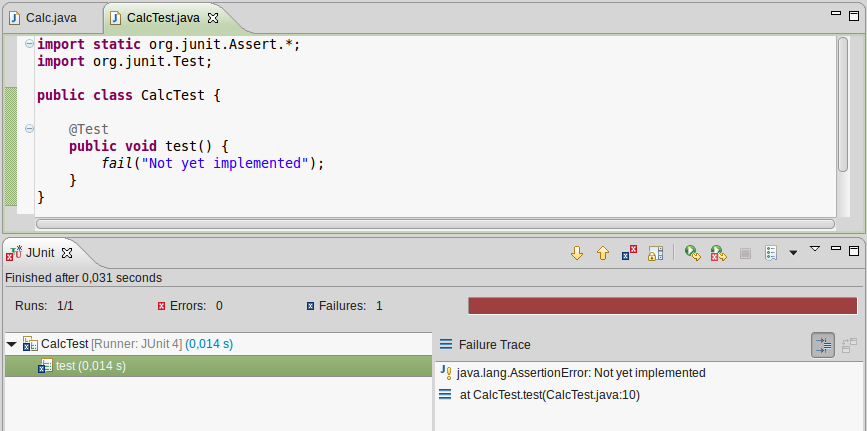
\includegraphics[scale=.3]{res/testing_fail.png}
\end{frame}

\subsection{Writing Tests}
\begin{frame}[fragile]{The first Test}
	\texttt{assertTrue()} checks if the condition is true. \\
	\texttt{assertFalse()} checks if the condition is false.
	\begin{lstlisting}[basicstyle=\ttfamily\scriptsize, escapechar=!]
	import static org.junit.Assert.*;
	import org.junit.Test;

	public class CalcTest {

	    @Test
	    public void testNormalAddition() {
	        Calc calc = new Calc();
	        assertTrue(calc.add(3, 5) == 8);
	        assertFalse(calc.add(3, 5) == 0);
	    }
	}
	\end{lstlisting}
	If and only if all assert methods add up the test will succeed.
\end{frame}

\begin{frame}[fragile]{Classic Import}
	If you use \emph{import} instead of \textbf{import static} you have to call 
	the assert methods via \emph{Assert.assertTrue()} instead of \textbf{assertTrue()}.
	\begin{lstlisting}[basicstyle=\ttfamily\scriptsize, escapechar=!]
	import org.junit.Assert;
	import org.junit.Test;

	public class CalcTest {

	    @Test
	    public void testNormalAddition() {
	        Calc calc = new Calc();
	        Assert.assertTrue(calc.add(3, 5) == 8);
	        Assert.assertFalse(calc.add(3, 5) == 0);
	    }
	}
	\end{lstlisting}
\end{frame}

\begin{frame}[fragile]{Multiple Tests}
	You can put multiple tests in one test class.
	\begin{lstlisting}[basicstyle=\ttfamily\scriptsize, escapechar=!]
	public class CalcTest {

	    @Test
	    public void testNormalAddition() {
	        Calc calc = new Calc();
	        assertTrue(calc.add(3, 5) == 8);
	    }

	    @Test
	    public void testNegativeAddition() {
	        Calc calc = new Calc();
	        assertTrue(calc.add(3, -5) == -2);
	    }
	}
	\end{lstlisting}
\end{frame}

\begin{frame}[fragile]{Fixture - Before}
	A method annoted with \textbf{@Before} will run before the test methods. \\
	Use a method to set up an environment for the tests. \\
	Now the tests will become smaller and easier to read.
	\begin{lstlisting}[basicstyle=\ttfamily\scriptsize, escapechar=!]
	public class CalcTest {
	
	    private Calc calc;
	    
	    @Before
	    public void init() {
	        this.calc = new Calc();	    
	    }
	    
	    @Test
	    public void testNormalAddition() {
	        assertTrue(this.calc.add(3, 5) == 8);
	    }
	}
	\end{lstlisting}
\end{frame}

\begin{frame}[fragile]{Fixture - After}
	A method annoted with \textbf{@After} will run after the test methods. \\
	Use the method if there are things to tidy up:
	\begin{itemize}
		\item close database connections
		\item close file streams
		\item delete test databases or test files
	\end{itemize}
\end{frame}

\subsection{Testing Exceptions}
\begin{frame}[fragile]{Example Bookshelf}
	\begin{lstlisting}[basicstyle=\ttfamily\scriptsize]
	public class Bookshelf {
	
	    private String[] books;
	
	    public Bookshelf () {
	        this.books = new String[10];
	        this.books[0] = "Harry Potter";
	    }

	    public String getBook(int number) {
	       return this.books[number];
	    }
	}
	\end{lstlisting}
\end{frame}

\begin{frame}[fragile]{Test Bookshelf}
	If your software throws exceptions you have to verify the proper throwing of these exceptions.
	\begin{lstlisting}[basicstyle=\ttfamily\scriptsize, escapechar=!]
	public class BookshelfTest {
	
	    private Bookshelf bookshelf;

	    @Before
	    public void init() {
	        this.bookshelf = new Bookshelf();
	    }

	    @Test(expected = ArrayIndexOutOfBoundsException.class)
	    public void testOutOfBounds() {
	        this.bookshelf.getBook(15);
	    }
	}
	\end{lstlisting}
\end{frame}

\begin{frame}[fragile]{Test Bookshelf - in Detail}
	\begin{lstlisting}[basicstyle=\ttfamily\scriptsize, escapechar=!]
	@Test(expected = ArrayIndexOutOfBoundsException.class)
	public void testOutOfBounds() {
	    this.bookshelf.getBook(15);
	}
	\end{lstlisting}
	\vfill
	\texttt{expected} has to be a subclass of the interface \emph{Throwable}.
	\vfill
	\texttt{ArrayIndexOutOfBoundsException\textcolor{red}{.class}} shows the class of the exception
	the test expects to be thrown.
	\vfill
	There is no assert method needed in this test case.
\end{frame}

\subsection{Additional Information}
\begin{frame}{Why Unit Testing?}
	Unit tests do not need human interaction. The automation of testing needs less time than testing by hand. \\
	It is easy to rerun the tests when software is altered.
\end{frame}

\begin{frame}{Links}
	JUnit Javadoc: \\
	\url{http://junit.org/javadoc/latest/index.html}
	\vfill
	An extensive JUnit tutorial:
	\url{http://www.vogella.com/tutorials/JUnit/article.html}
\end{frame}
\end{document}